
Za razmijevanje potreba penjača potrebno je analizirati alate koje penjači koriste. Ta rješenja mogu se podijeliti u dvije glavne kategorije: tradicionalne tiskane vodiče i moderne digitalne platforme koje su odgovorile na neka od ograničenja tiskanih vodiča.

\subsection{Tradicionalni tiskani penjački vodiči}

Desetljećima su tiskani vodiči bili jedini dostupni izvor informacija za snalaženje na stijenama. Njihova temeljna vrijednost leži u detaljnom i strukturiranom prikazu informacija koje kreiraju iskusni penjači. 

Vodiči su gotovo uvijek organizirani hijerarhijski kako bi korisniku olakšali navigaciju. Na najvišoj razini, vodič je podijeljen na šira penjačka područja, primjerice Kalnik, Kanjon Čikola, Golubinjak. Ta penjačka područja su često označena na velikoj karti koja se nalazi na početku vodiča. Unutar svakog područja sadržaj se dalje raščlanjuje na pojedinačne sektore, odnosno manje odvojene dijelove stijene. Za svaki sektor pružaju se ključne logističke informacije poput detaljni opis prilaza, informacije o parkiranju, vrijeme potrebno za pristup, GPS koordinate te opće napomene poput osunčanost ili preporučeno doba godine za posjet. 
Središnji element svakog vodiča je vizualni prikaz smjerova, odnosno \textit{topo}, koji može biti u formi detaljnog crteža ili fotografije preko koje su ucrtane linije smjerova. Uz svaki smjer navode se podaci o smjeru poput naziv, težina, dužina smjera te eventualno napomene poput upozorenje na nestabilno kamenje sklono kidanju. Osim informativnih \textit{topo} prikaza, vodiči su često obogaćeni fotografijama penjača te pejzažnim forografijama. 


U pravilu svaki vodič pokriva specifično geografsko područje, od pojedinačnog velikog penjališta do cijele regije. U Hrvatskoj, najpoznatiji primjer vodiča za veću regiju je vodič "Croatia" autora Borisa Čujića. Uz njega postoje i specijalizirani vodiči za pojedina područja poput Nacionalnog parka Paklenica ili za regiju Istre.

\begin{figure}[H]
    \centering
    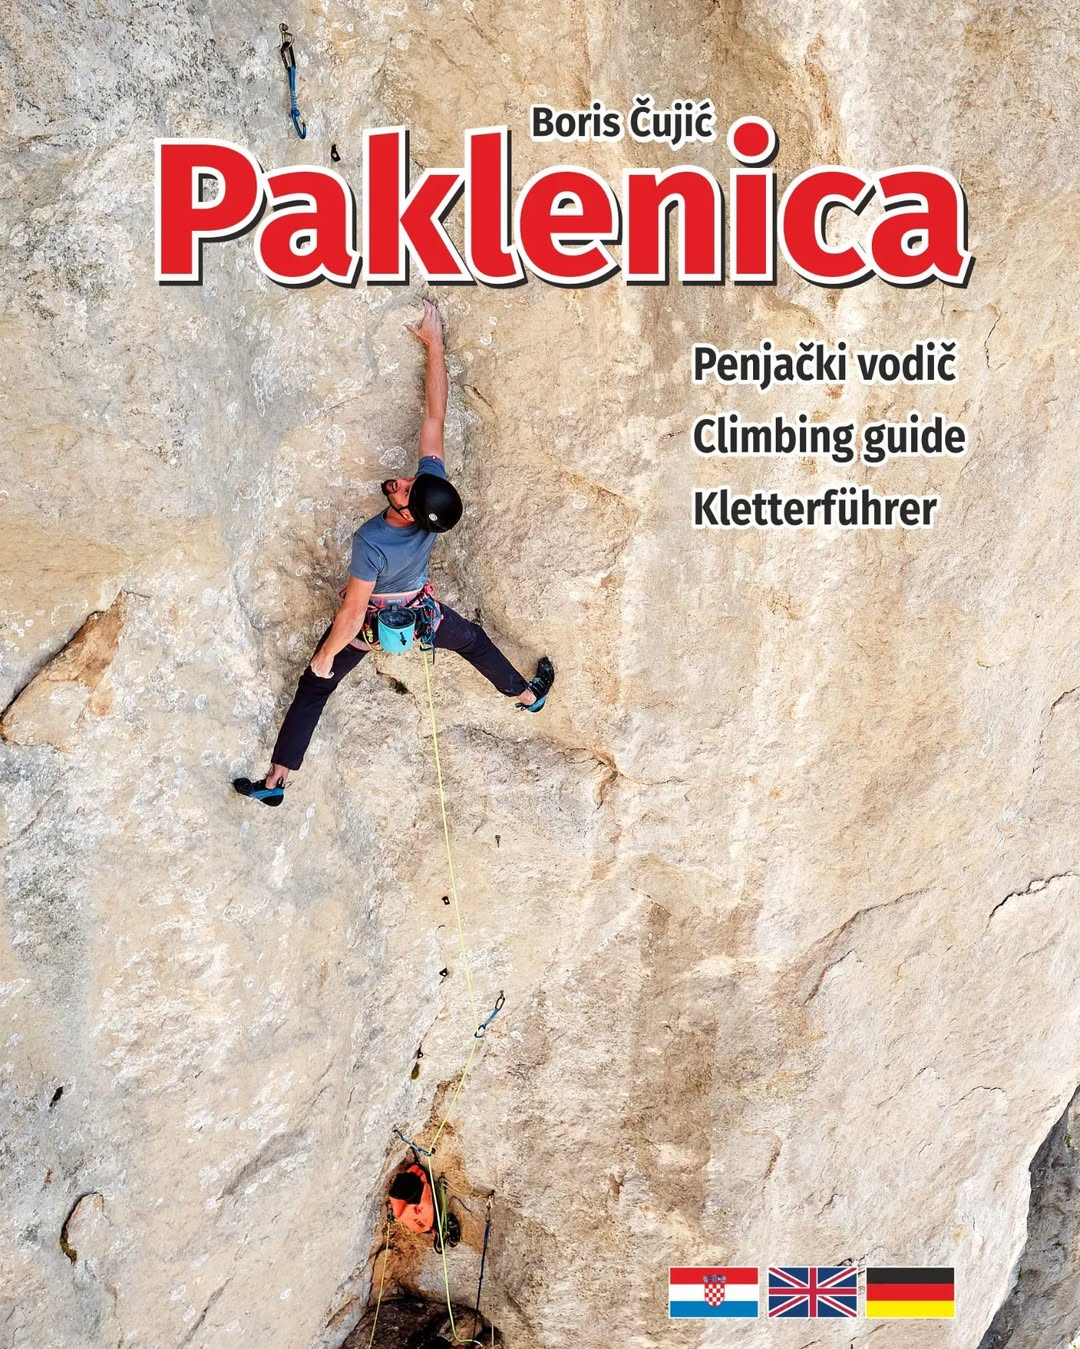
\includegraphics[width=0.6\textwidth]{images/analiza/vodic_paklenica.jpeg}
    \caption{Prikaz tiskanog penjačkog vodiča "Paklenica" autora Borisa Čujića}
\end{figure}

Dodatnu složenost unose i izdanja stranih izdavača poput "Istra" autora Jurija Ravnika. Ova raznolikost izdavača dovodi do nedostatka konzistentnosti. Različiti vodiči koriste različite simbole, stilove i metodologije izrade \textit{topo} skica. Neki se oslanjaju na ručno crtane skice, a neki na fotografije. Bitno je spomenuti da se neujednačenost vidi i u težinama smjerova. Nije rijetko da isti smjer ima različite težine u različitim vodičima, što nije nužno posljedica promjene na stijeni ili novije izdanje, već subjektivna procjena autora. Ponekad se dogode i veće pogreške pri određivanju težine smjera što može dovesti do zabune. Sveukupno te nekonzistentnosti otežavaju snalaženje penjačima koji posjećuju različita područja i koriste vodiče različitih autora. 




\subsection{Digitalne platforme}

Ograničenja u tiskanim vodičima dovela su do pojave digitalnih platformi koje su omogućile veću dostupnost i ažurnost podataka. Dvije platforme, 8a.nu i 27crags, ističu se kao primjer rezličitih pristupa unutar digitalnog penjačkog svijeta. 

\subsubsection{8a.nu}

Platforma 8a.nu pokrenuta je 2000.\ godine i predstavlja jednu od najstarijih digitalnih platformi za penjanje. Njena glavna svrha nije funkcija terenskog vodiča, već uloga globalnog dnevnika uspona i sustava za rangiranje. Korisnici koriste platformu kako bi bilježili svoje ispenjane smjerove, navodeći stil uspona, predlagajući težine i komentare za smjerove. Time se stvara velika, iako često nestrukturirana, baza podataka koja služi kao arhiv i statički resurs.

\begin{figure}[H]
    \centering
    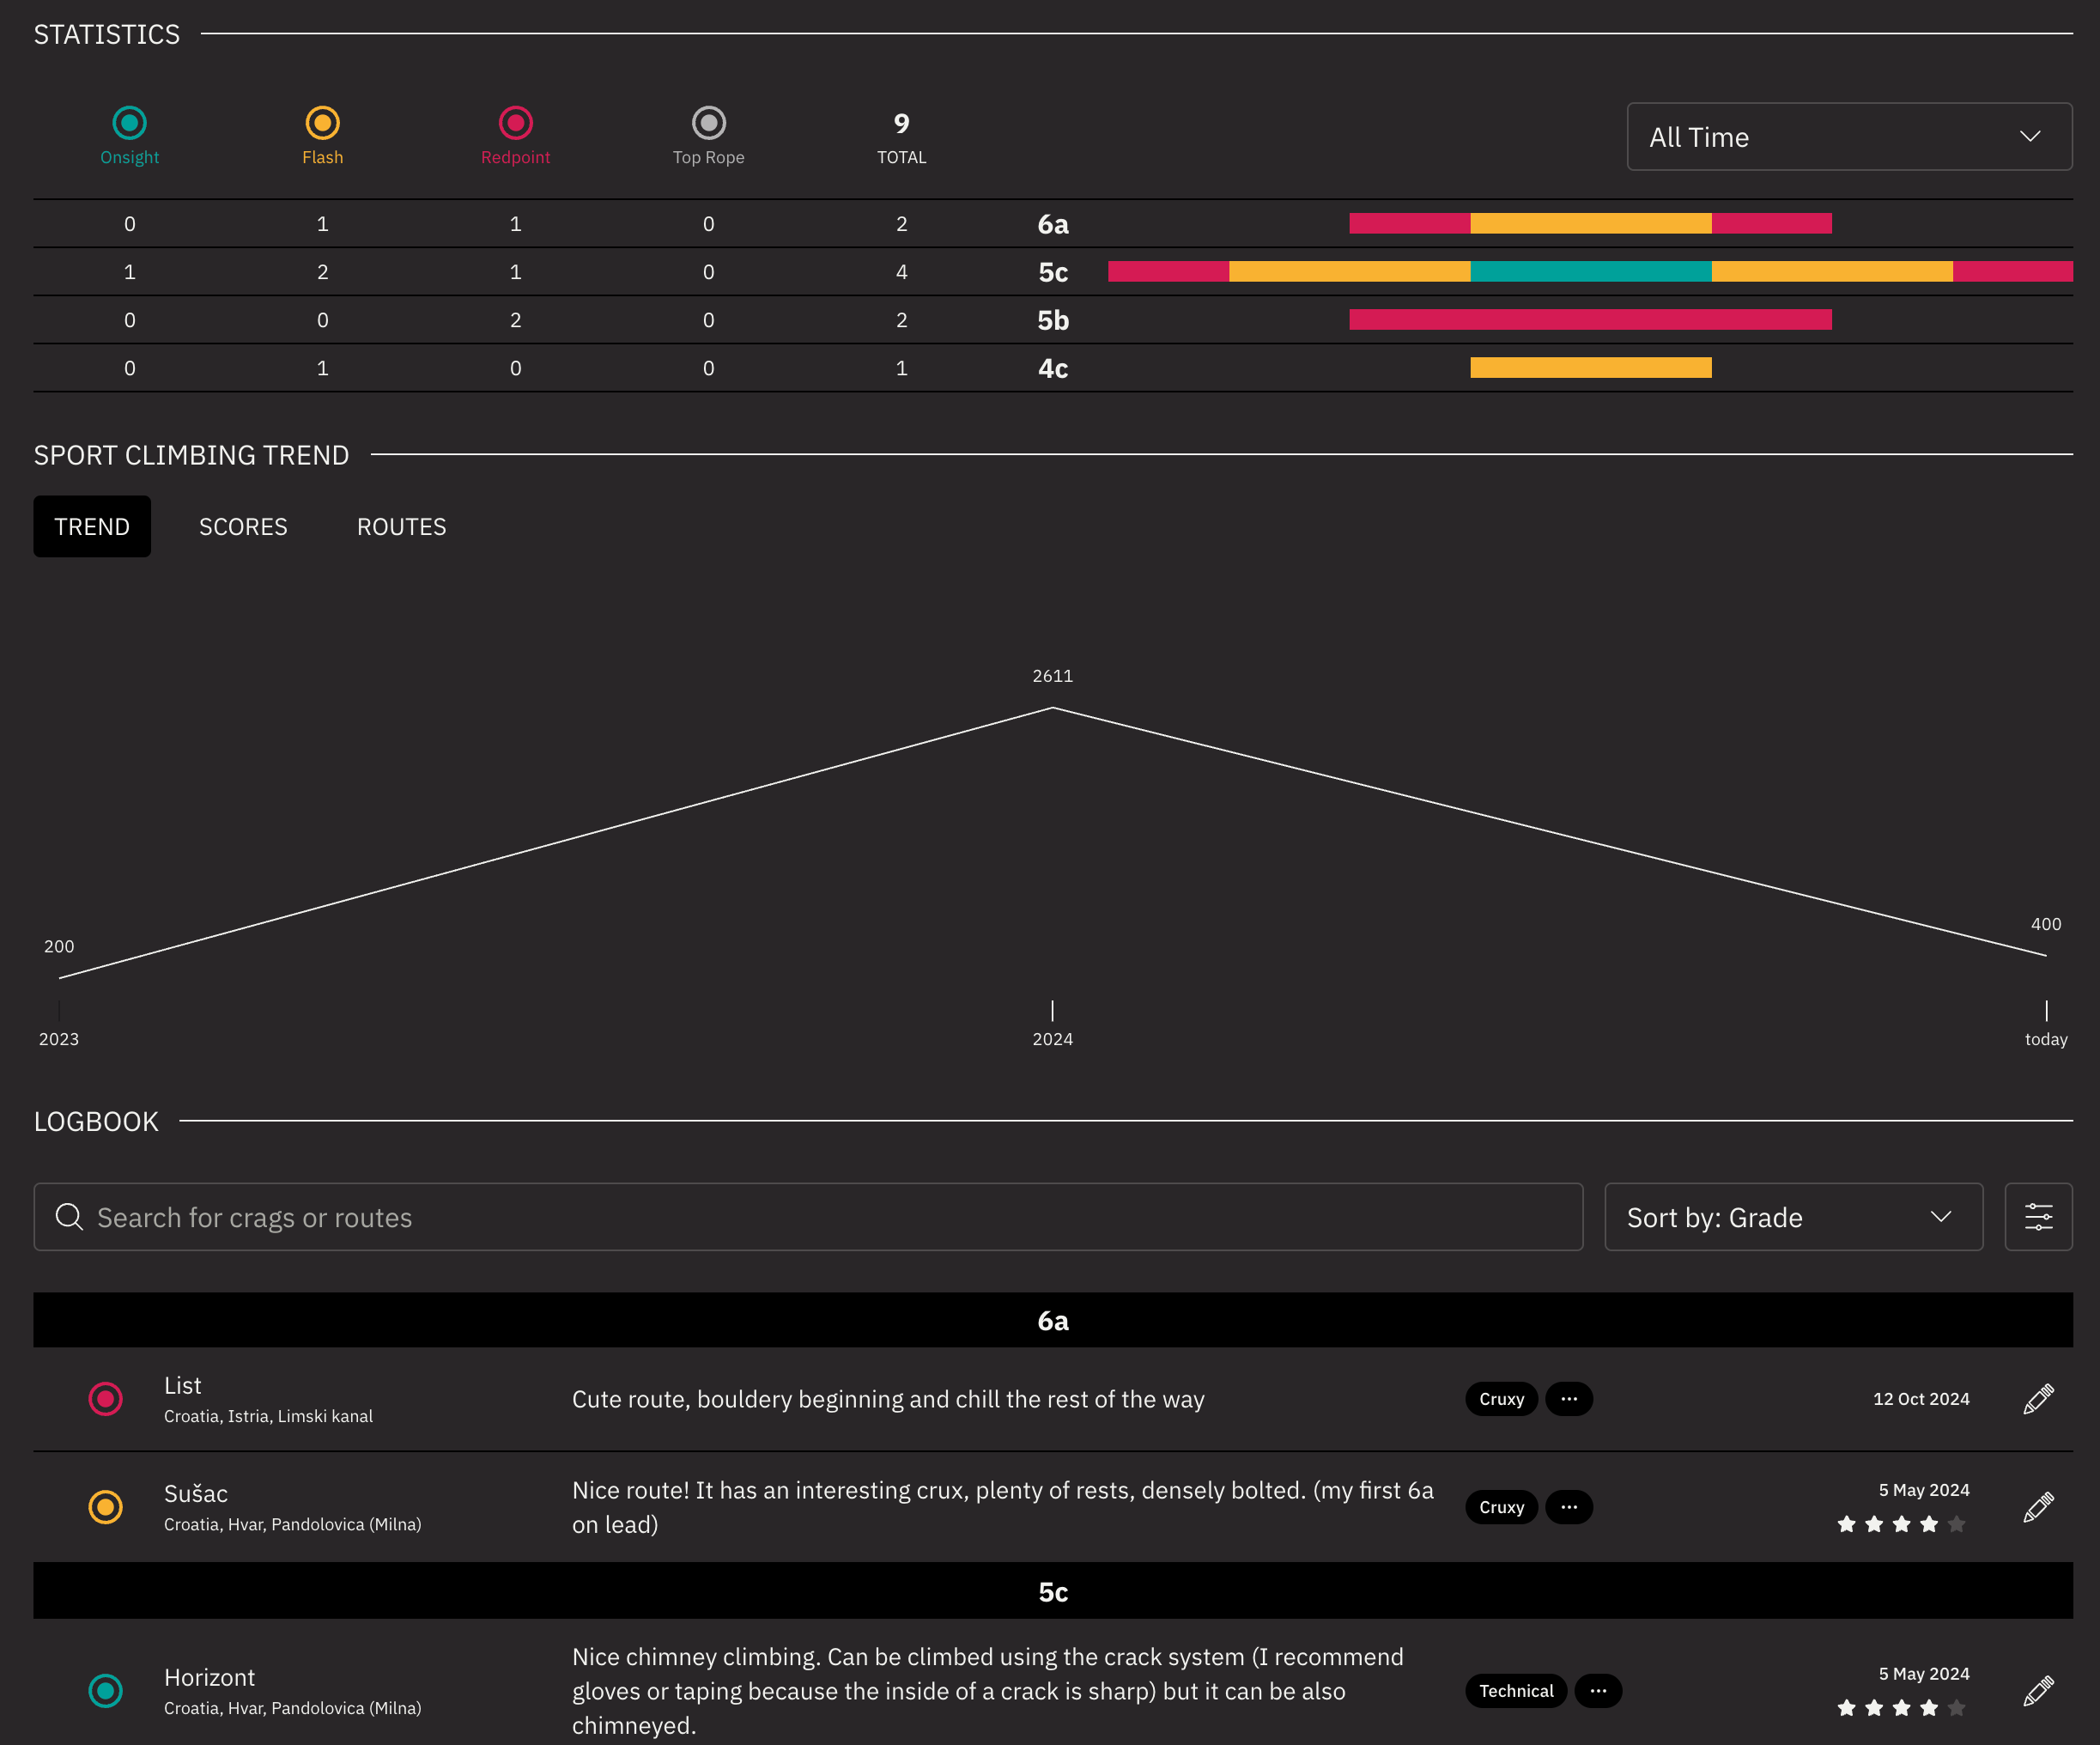
\includegraphics[width=0.8\textwidth]{images/analiza/8anu_logbook.png}
    \caption{Prikaz dnevnika uspona na platformi 8a.nu}
\end{figure}

Ta društvena i natjecateljska komponenta je razlog njene dugovječnosti jer motivira penjače svih razina da upisuju svoje uspone. Platforma također nudi vjesti o značajnim usponima i forum za raspravu između penjača. Unatoč što aplikacija nudi \textit{topo} slike i hijerarhijski organizirane penjačke lokacije, njena primarna uloga je i dalje orijentirana prema društvenom aspektu. 
S nedavnim razvojem mobilne aplikacije, platforma je modernizirala korisničko sučelje i poboljšala dostupnost podataka na terenu nudeći opciju preuzimanja podataka na lokalni uređaj. Time je sustav upotrijebiv i u uvjetima bez signala.


\begin{figure}[H]
    \centering
    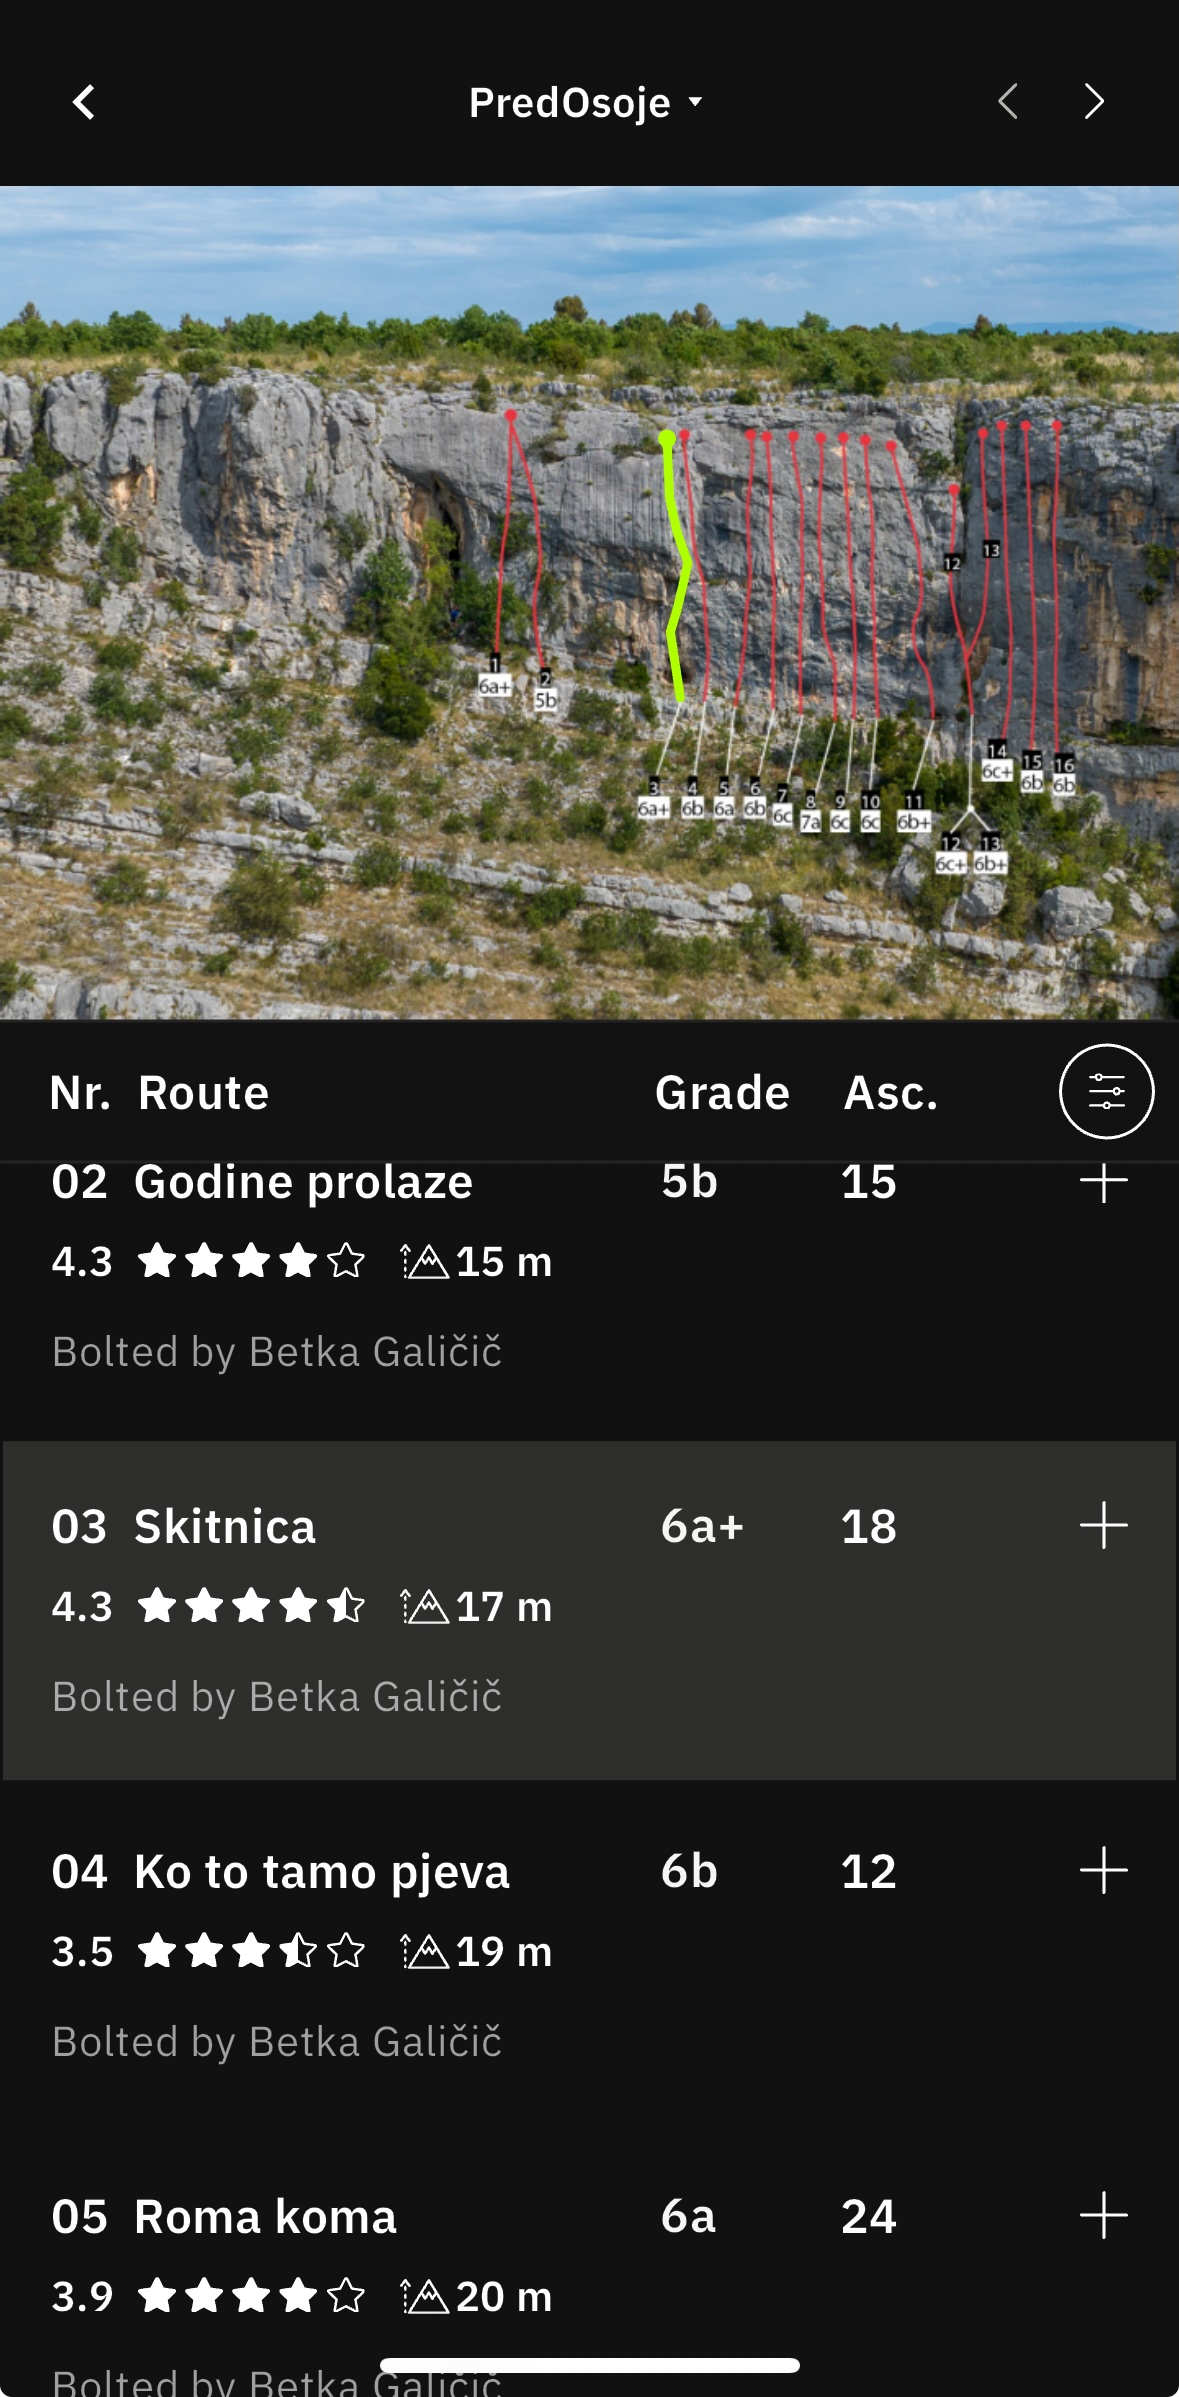
\includegraphics[width=0.4\textwidth]{images/analiza/8anu_mobile.jpg}
    \caption{Prikaz \textit{topo} skice na mobilnoj aplikaciji 8a.nu}
\end{figure}


Analizirajući 8a.nu kao alata za snalaženje na stijeni, njeni nedostaci u kontekstu vizalne navigacije su i dalje prisutni. Temeljni problem leži u samoj prirodi vizalnih prikaza. \textit{Topo} fotografije su često snimljene s velike udaljenosti kako bi obuhvatile cijeli sektor, zbog čega su ucrtane linije smjerova malene i nejasne. Ovaj problem postaje posebno izražen na sektorima s velikom gustoćom smjerova, kao što je prikazano na primjeru sektora PredOsoje, gdje je teško precizno raspoznati pojedinačne linije i njihove početke. Dodatni problem predstavlja i neujednačena pokrivenost. Dok su međunarodno popularna penjališta dobro dokumentirana, manje ili lokalne penjačke lokacije, poput Kalnika u Hrvatskoj, nemaju dostupne \textit{topo} prikaze. Unatoč svojoj važnosti kao arhiva, 8a.nu nije pouzdano rješenje za problem identifikacije smjerova na stijeni.

\subsubsection{27crags}

27crags predstavlja digitalnu platformu za penjače koje je izrađeno primarno s ciljem pružanja informacija o penjačkim lokacijama i smjerovima. Ideja platforme 27crags je popisati što više penjačkih lokacija i smjerova, a manji fokus je stavljen na društveni aspekt. \textit{Topo} skice su napravljene na sličan način kao i kod 8a.nu, no društveni aspekt po pitanju uspona drugih penjača nije toliko u fokusu kao kod 8a.nu. Aplikacija nudi više informacija o penjačkoj lokaciji, poput parking lokacije sa detaljnim kartografskim prikazom.

Unatoč boljoj pokrivenosti penjačkih lokacija, 27crags također ima limitacije po pitanju dvodimenzionalnog \textit{topo} prikaza čime se ne riješava problem identifikacije penjačkih smjerova.

\begin{figure}[H]
    \centering
    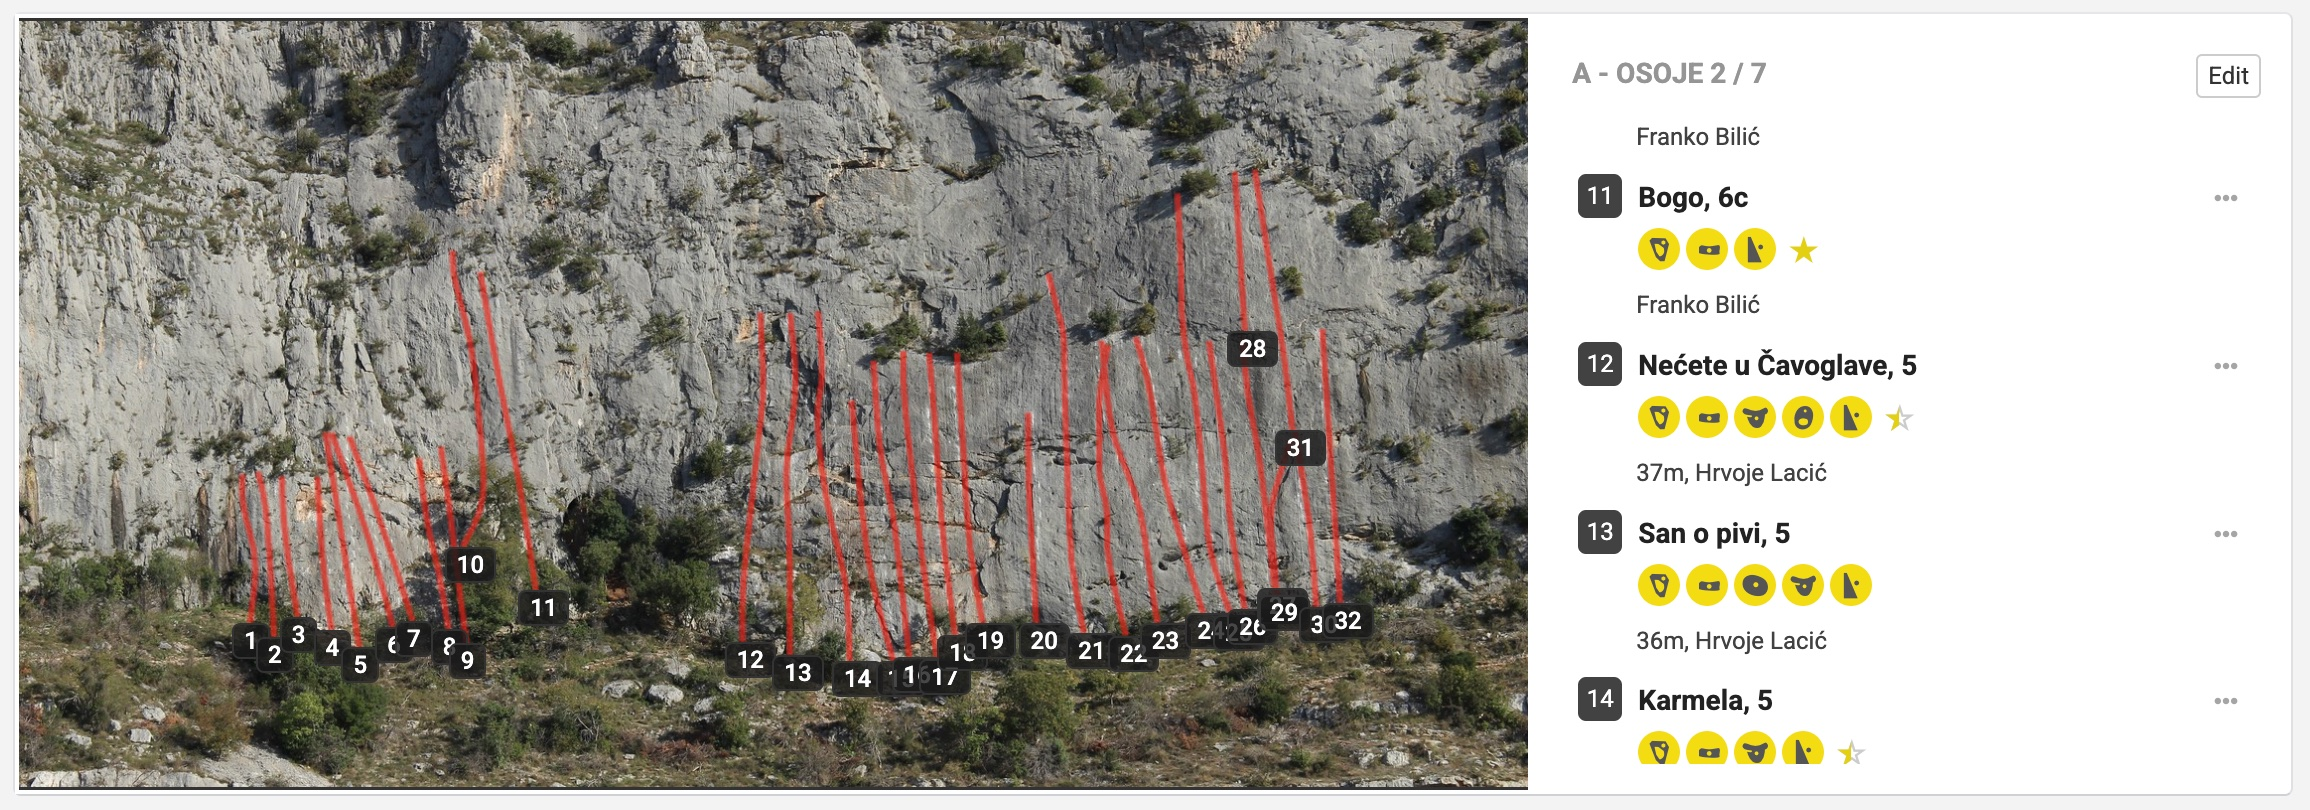
\includegraphics[width=0.75\textwidth]{images/analiza/cikola_27crags_topo.jpeg}
    \caption{Prikaz dvodimenzionalne \textit{topo} skice sa 27Crags za penjalište Čikola sektora Osoje}
\end{figure}

\begin{figure}[H]
    \centering
    \includegraphics[width=0.65\textwidth]{images/analiza/cikola_fizicka_slika.jpg}
    \caption{Stvarna stijena na penjalištu Čikola sektora Osoje}
\end{figure} 